\documentclass[runningheads]{llncs}
%
\usepackage[T1]{fontenc}
\usepackage{graphicx}
\usepackage{caption}
\usepackage{float}
\usepackage{listings}
\lstset{
    basicstyle=\ttfamily,
    columns=fullflexible,
    breaklines=true,
    frame=single,
    showtabs=false,
    tabsize=2,
    captionpos=b
}
%
\begin{document}

\begin{figure}[t]
\centering
\includegraphics[width=7cm]{images/logo.png}  % Adjust width as needed
\end{figure}
\vspace{-1cm}  % Adjust vertical spacing

\title{Crowd Evacuation Dynamics at Sporting Events: A Simulation using GAMA Platform}

\author{Christian Faccio \and Javier Arribas González \and Luis Bernabeu Agüeria \and Imanol Jurado Martínez \and Bruno Sancho Deltell}

\institute{University of Alicante}

\maketitle

\begin{abstract}
    Crowd evacuation from large buildings is a critical aspect of public safety, especially during emergencies. This problem can be well modeled using agent-based models (ABM), where individuals are represented as autonomous agents with specific behaviors and interactions. Simulations can then be made to analyze evacuation dynamics and optimize safety protocols. This report presents the StadiumEvacuation model, an ABM developed using the GAMA platform \cite{taillandier2018gama}, which simulates crowd evacuation in a stadium environment under the threat of a spreading hazard. A snapshot of the simulation is shown in Fig.\ref{fig:1}.
\end{abstract}
     
\section{Project context and goals}

The \textit{StadiumEvacuation} model is an agent-based simulation designed to study crowd evacuation dynamics inside a stadium-type environment when a spreading hazard (for example, a flood or fire front) threatens people's safety. The model's top-level intent is to reproduce how individual decision-making, local interactions, staff presence, and stadium geometry combine to produce system-level outcomes (number saved, number of victims, spatial bottlenecks).  

Parameters are exposed globally so experiments can sweep them: total population, relative number of workers, perceptual ranges, movement speed, hazard speed ratio, and behavioral composition. The model therefore targets sensitivity analysis and “what-if” testing (how many workers, how long perception ranges, how fast hazard spreads) to inform design or management decisions.

To model the problem we used ABM: each human is an autonomous agent (spectator or worker) with perceptions, beliefs, desires and simple plans (a lightweight BDI-like control). The physical layout is read from GIS shapefiles so the geometry is realistic: roads (navigable network), buildings (obstacles) and evacuation points (exits). A single hazard agent expands its shape over time and “covers” agents, which then become victims. The model records per-role and per-type data to enable detailed post-run analysis. 

\begin{figure}[H]
\centering
\includegraphics[width=\textwidth]{images/snapshot.png}  %Adjust width as needed
\caption{StadiumEvacuation model screenshot showing agents evacuating the stadium while a hazard (red area) spreads.}
\label{fig:1}
\end{figure}

\section{Spatial environment and representation}

The environment is based on GIS data. The model expects three shapefiles under the \texttt{../includes/} folder: \texttt{paths.shp} (roads), \texttt{buildings.shp} (buildings) and \texttt{exits.shp} (evacuation points). These layers are used to build the world geometry and navigation infrastructure. The code creates \texttt{road}, \texttt{building} and \texttt{evacuation\_point} species from those files in the \texttt{init:} section.

The geometry shape is computed as the envelope of the union of the three layers:
\begin{lstlisting}
geometry_shape <- envelope(envelope(road_file)+envelope(buildings)+envelope(evac_points));
\end{lstlisting}
    
Roads, instead, are converted to a graph structure to enable agent navigation:

\begin{lstlisting}
road_network <- as_edge_graph(road);
\end{lstlisting}

This graph is used by agents for pathfinding (\texttt{do goto target: safety\_point on: road\_network speed: speed;}), which produces realistic movements.
\newpage
The code thus implies some design considerations and expectations:
\begin{itemize}
    \item The \texttt{paths.shp} layer should provide a fully connected navigation network. Every intersection between overlapping lines has been manually defined using the QGIS software \cite{QGIS_software}. If the network contains disconnected components, some agents may start in areas with no path to the exits. The code assigns \texttt{safety\_point <- evacuation\_point closest\_to(self)}, but if there’s no route to that point, the agent’s \texttt{goto} command may fail or take unrealistic Euclidean shortcuts depending on the simulator;
    \item \texttt{evac\_points} should be positioned so agents can reach them from roads (snapping or nearest-node logic is necessary if shapefiles are slightly misaligned);
    \item Coordinate Reference System (CRS) consistency is assumed for the three shapefiles; mismatched projections will produce incorrect distances and routing.
\end{itemize}

The environment is also visualized: the three species \texttt{road}, \texttt{building} and \texttt{evacuation\_point} define aspect default drawing rules (colors, borders), and evacuation points draw themselves with a radius that reflects the number of saved agents close to them (\texttt{count\_exit\_spectators}, \texttt{count\_exit\_workers}), which is a visual feedback mechanism for flows through exits.

\section{Agent design, internal states and behaviors}

The model implements three species with clear and defined responsibilities: \texttt{spectator}, \texttt{worker} and \texttt{hazard}. Spectators and workers both have mobility and decision logic; workers are specialized leaders. The code uses reflexes as plans (BDI-like constructs since using a complete BDI crashes the model using 1000+ agents) to capture perception $\to$ decision $\to$ action cycles. Now we are going to describe attributes and behavior mechanisms in detail and implementation concepts that are necessary to understand how the model works.

\subsection{Spectators}

Spectators represent the core of the population within the \texttt{StadiumEvacuation} model, embodying the collective dynamics of ordinary individuals attending a large-scale event. Their behavior is modeled at the individual level, where each spectator acts as an autonomous agent capable of \textit{perceiving}, \textit{reacting}, and \textit{influencing} others in their surroundings. In the simulation, spectators are not passive entities but decision-makers operating under limited information, perception constraints, and social influences, features that collectively generate emergent crowd behavior.

\subsubsection{Initialization and Spatial Distribution}

At the beginning of each simulation run, a defined number of spectators (\texttt{nb\_of\_spectators}) is created according to the total population (\texttt{tot\_people}) and the ratio of workers to spectators (\texttt{workers\_over\_spectators}). Each spectator is placed at a random position within the road network, ensuring that agents start from realistic and accessible areas within the stadium.

In the code, this initialization is achieved through:

\begin{lstlisting}
create spectator number:nb_of_spectators {
    location <- any_location_in(one_of(road)); 
    safety_point <- evacuation_point closest_to(self);
    perception_distance <- rnd(min_perception_distance, max_perception_distance); 
}
\end{lstlisting}

This means that each spectator receives an individualized exit target (\texttt{safety\_point}), the nearest evacuation point defined in the GIS layer, and a randomized perception distance, which controls how far they can detect the hazard or observe others reacting. These parameters introduce natural variability, reflecting differences in attention, awareness, and spatial orientation among real people.

\subsubsection{Behavioral Typologies: Leaders, Followers, and Panic Agents} 

The population of spectators is intentionally heterogeneous, composed of three behavioral archetypes that define how each agent perceives and reacts to the situation:
\begin{itemize}
    \item \textbf{Leaders}: proactive individuals who tend to take initiative when danger arises. They react faster to the hazard, influence others through example, and contribute to the formation of organized evacuation fronts;
    \item \textbf{Followers}: reactive individuals who depend heavily on social observation. They begin to move only after noticing others (leaders, workers, or alerted neighbors) reacting to the threat;
    \item \textbf{Panicked}: individuals overwhelmed by the situation. They act erratically, move less efficiently, and can even slow down surrounding agents by creating local turbulence or congestion.
\end{itemize}

This differentiation is implemented stochastically at initialization:
\begin{lstlisting}
float r <- rnd(1.0);
    
if (r < leader_frac) {
    role <- "leader";
} else if (r < (leader_frac + follower_frac)) {
    role <- "follower";
} else {
    role <- "panic";
    perception_distance <- 1.0;
}
\end{lstlisting}

Here, \texttt{leader\_frac} and \texttt{follower\_frac} are adjustable global parameters that determine the composition of the crowd, while the remaining fraction corresponds to panic agents. Panic individuals are assigned a fixed short perception range (1.0 meter), representing their reduced situational awareness.

\subsubsection{Perception and Alert Propagation} Spectators do not initially know that a hazard exists. They begin in a “watching” state, unaware of any danger. The transition from ignorance to alertness occurs through perception-based interactions. Each spectator regularly checks its surroundings for two triggers:
\begin{itemize}
    \item Direct perception of the \textbf{hazard}, if it enters their perception radius;
    \item Observation of \textbf{alerted agents} (either workers or spectators already reacting).
\end{itemize}

This mechanism is captured by the reflex:
\begin{lstlisting}
// Check for nearby alerted spectators
list<spectator> nearby_alerted <- (spectator at_distance perception_distance) where (each.being_alerted);
if not empty(nearby_alerted) {
    being_alerted <- true;
    do remove_belief(not_alerted);
    do add_belief(alerted);
    do remove_desire(watch);
    do add_desire(predicate: escape, strength: 5.0);
}
\end{lstlisting}

When triggered, the agent’s internal state changes, it removes the \texttt{not\_alerted} belief, adds the \texttt{alerted} belief, and replaces the \texttt{watch} desire with an \texttt{escape} desire of higher strength. This chain of changes follows the \textbf{Belief-Desire-Intention (BDI)} cognitive model, a simple but effective decision framework used in agent-based systems to simulate human reasoning. As a result, awareness spreads organically through the crowd, resembling a social contagion process where individuals influence each other’s perception of risk.

\subsubsection{Movement and Navigation Dynamics}

Once alerted, spectators initiate movement toward their assigned evacuation point. Navigation occurs on the road network graph, generated from the GIS path data. Agents use GAMA’s \texttt{goto} command with the parameter on: \texttt{road\_network}, which ensures pathfinding along connected routes and prevents crossing through walls or restricted areas.

\begin{lstlisting}
reflex move_to_safety when: being_alerted and not (saved or drowned) {
    do goto target: safety_point on: road_network speed: speed;
}
\end{lstlisting}

\texttt{speed} is a dynamic attribute influenced by both crowd density and psychological state. Each agent’s velocity is adjusted depending on how many others are within its perception radius, a mechanism that reproduces congestion effects:
\begin{lstlisting}
    speed <- speed * (0.5 + 0.5 * exp(-exp_weight * n_people));
\end{lstlisting}

As local density increases, this expression reduces the effective speed, simulating how individuals naturally slow down when surrounded by large groups.

Additionally, roles exert \textit{social influence} on the movement of nearby agents. Leaders increase the speed of those around them, promoting more decisive motion, whereas panic agents decrease it, symbolizing confusion and hesitation. This feedback mechanism creates self-organizing evacuation flows, where zones dominated by leaders clear faster while areas with panic individuals tend to clog.

\subsubsection{Hazard Interaction and Outcome Tracking}

The interaction between spectators and the hazard defines the critical outcome of the evacuation. The hazard spreads outward from an initial point as an expanding front, representing elements like fire, smoke, or flooding. As it advances, spectators must move toward their designated exits before being overtaken.

Each step, the model checks whether a spectator’s position overlaps with the hazard. If so, the agent is marked as drowned, removed from the simulation, and the global and role-specific victim counters are updated. Conversely, when an agent reaches its safety point, it is marked as saved, and similar counters track successful evacuations.

These two outcomes , drowning or escaping , form the terminal states of every spectator. Together, they provide quantitative indicators of evacuation efficiency and risk. By analyzing the ratios of survivors to victims across behavioral types and scenarios, researchers can evaluate how leadership, panic, perception, and spatial factors influence overall safety and the effectiveness of evacuation strategies.

\subsubsection{Emergent Behavior and Interpretation}

Through these mechanisms, the spectators collectively produce complex and realistic evacuation dynamics. Local rules , such as limited perception, social influence, and adaptive speed , generate emergent phenomena like \textbf{bottlenecks}, \textbf{wave-like evacuation fronts}, and \textbf{nonlinear reaction patterns}.

For example, in regions with many panic agents, the flow slows dramatically, creating clusters of congestion that delay evacuation even for individuals who are otherwise capable of escaping. Conversely, when leaders or workers dominate a region, movement becomes more organized and efficient, reducing overall evacuation time.

The spectator system thus represents the emergent social dimension of the evacuation process. While each agent follows simple behavioral rules, their interactions yield global outcomes that mirror the complexity of real human crowds. By varying parameters such as the ratio of leaders to followers, perception ranges, or total population size, researchers can explore a wide range of scenarios , from orderly evacuations to chaotic panics ,  and analyze how individual diversity shapes collective safety outcomes.

\subsection{Workers}

Workers represent trained staff or security personnel responsible for guiding spectators during evacuation. Structurally similar to spectators, they differ in that each worker begins the simulation as a leader and in an alerted state, automatically adopting the escape desire. Their perception distance is randomly assigned, defining how far their influence extends.

Conceptually, workers act as mobile sources of order and information, helping to spread awareness and promote faster responses among nearby spectators. Through the \texttt{role\_influence} reflex, they increase the speed of surrounding agents, enhancing group coordination and reducing panic effects.

They move deterministically along the \texttt{road\_network} toward their assigned \texttt{safety\_point}, never exhibiting chaotic or panic-driven behavior. When reached by the hazard, they are recorded as victims; when safe, they increment the saved counters before being removed. Overall, workers embody the guiding and stabilizing force of the evacuation, crucial for efficient collective movement under hazard pressure.

\subsection{Hazard}

The hazard represents an expanding threat, such as fire or smoke, that starts from a random point within the stadium and grows outward over time. Its spread rate is determined by a predefined propagation speed, calculated as a multiple of the agents’ movement speed. This allows realistic control of how quickly the danger evolves relative to human mobility.

Visually displayed as a semi-transparent red area, the hazard expands continuously but remains confined within the simulated environment. Its speed is recalculated at initialization to ensure consistency across experiments. Overall, it functions as the primary environmental pressure driving agent behavior and evacuation dynamics, influencing both decision-making and final outcomes.

\section{Experiments}

\subsection*{1: Impact of Worker to Spectator Ratio on Evacuation Success}

This experiment takes into consideration two parameters:
\begin{itemize}
    \item Total number of people;
    \item Worker over Spectator ratio.
\end{itemize}

A batch simulation was configured in GAMA to test these parameters for a range of values (from $500$ to $1500$ for total people, and from $0.2$ to $1.0$ for worker over spectator ratio), with $10$ repetitions for each combination of parameters. The main metric tracked was the overall survival rate, calculated as the percentage of people who managed to evacuate successfully. As shown in Fig.\ref{fig:exp1_1}, as the total number of people increases, we should introduce more workers to have a good survival rate. That is quite intuitive, but with a simulation like this we can estimate both the required number of workers and the expected survival rate for each configuration. 

\begin{figure}{h}
\centering  
\includegraphics[width=0.9\textwidth]{../analysis/output/1.2.png}
\captionof{figure}{Figure shows evacuation simulation results across varying population sizes (500-1500 people) and worker-to-spectator ratios (0.2-1.0). (a) Survival rate increases with worker ratio across all population sizes, with smaller populations showing steeper improvements. (b) Larger populations generally achieve higher survival rates, particularly at higher worker ratios. (c) Contour map reveals optimal configurations in the upper-right region (high worker ratios, larger populations). (d) Best-performing scenarios cluster around high worker ratios (0.8-1.0) with populations of 1000-1500, achieving $95-98\%$ survival rates, while worst performers show low worker ratios (0.2-0.3) with 500-600 people, achieving only $52-58\%$ survival.}
\label{fig:exp1_1}
\end{figure}

Moreover, we can inspect the results in more detail, considering the sub-categories of the spectators and dividing between spectators and workers. As shown in Fig.\ref{fig:exp1_2}, overall the results are consistent with the previous analysis, but we can see that workers always have a better survival rate than spectators, which is expected since they are trained for these situations. Leaders also have a better survival rate than followers, which is also expected since they are the first to react to the hazard. Panic agents have the worst survival rate, but their impact on the overall survival is limited since they represent a small fraction of the population. At the end, given these results, we should focus on reducing the number of panic people since they are the ones that most negatively impact the overall survival rate.

\begin{figure}{h}
\centering  
\includegraphics[width=0.9\textwidth]{../analysis/output/1.1.png}
\captionof{figure}{Figure shows normalized evacuation outcomes as survival rates (\%) across population sizes (500-1500) and worker-to-spectator ratios (0.2-1.0). (a) Overall survival rate improves from $\approx 57\%$ to $\approx 97\%$ as worker ratio increases, with best performance at higher populations and ratios. (b) Leaders consistently achieve $60-75\%$ survival across configurations. (c) Followers show $55-75\%$ survival, improving significantly with higher worker ratios. (d) Panic agents represent $5-10\%$ of total population saved, decreasing slightly with higher worker ratios. (e) Spectator survival mirrors overall trends ($55-90\%$), improving with worker ratio and population size. (f) Workers consistently achieve $60-98\%$ survival, with dramatic improvements at higher ratios, demonstrating their trained advantage.}
\label{fig:exp1_2}
\end{figure}

\subsection*{2: Analysis of Max Perception Distance}

This experiment was designed to quantify the impact of the parameter \newline \texttt{max\_perception\_distance} on evacuation outcomes. A batch simulation was configured to test this parameter across a range from $200.0$ to $1200.0$, with $20$ repetitions per $100.0$-unit step. The primary metrics tracked were the mean overall survival rate, the standard deviation of survival (to measure variability), the mean number of panic victims, and the mean survival rate of agents who entered a panic state.

\begin{figure}
\centering  
\includegraphics[width=0.7\textwidth]{../analysis/output/2.png}
\captionof{figure}{Mean overall survival rate (\texttt{survival\_mean}) and standard deviation (\texttt{survival\_std}) across varying \texttt{max\_perception\_distance} values (200.0-1200.0).}
\label{fig:exp2}
\end{figure}

The results shown in Fig.\ref{fig:exp2} indicate a complex and non-linear relationship between perception distance and overall survival. Mean survival was lowest at minimal perception distances ($\approx 45\%$ at $200-400$), suggesting a baseline inability to locate exits. A significant improvement occurred at $500.0$ ($59.8\%$ mean survival), with a general performance peak observed between $600.0$ and $800.0$ ($63-64\%$). Notably, the trend was not linear; after a dip, the highest mean survival was recorded at $1100.0$ ($71.1\%$), which was immediately followed by a sharp performance drop at $1200.0$ ($47.5\%$). A critical finding across all settings was the high standard deviation ($18-26\%$), indicating that outcomes are highly stochastic and variable, even with identical parameters.

The analysis of panic-related metrics provided distinct insights. First, the mean number of panic victims (\texttt{panic\_victims\_mean}) remained relatively low and showed no clear correlation with perception distance, fluctuating between $3.0$ and $7.8$. This suggests that perception distance does not significantly influence the likelihood of an agent panicking. However, the \texttt{panic\_survival\_mean} (the survival rate of panicked agents) showed a clear positive trend. At low distances ($200-300$), panicked agents had a $78-85\%$ survival rate, which improved to a consistent $88-93\%$ at distances of $500.0$ and above. This implies that while increased perception doesn't prevent panic, it substantially improves the chances of survival for those who do.

\subsection*{3: Interaction of Agent Speed and Hazard Spread Rate}

This experiment evaluates how evacuation performance in the StadiumEvacuation model is affected by the interaction between human mobility and the speed at which the hazard spreads. The experiment systematically varies two key parameters: \texttt{Speed People} (ranging from $1.0$ to $10.0$) and \texttt{Speed Ratio} ($2.0$ to $5.0$, representing how many times faster the hazard expands compared to the agents). Each parameter combination is repeated 20 times,. This design provides a robust sensitivity analysis of how physical mobility and hazard pressure jointly determine evacuation outcomes.

For every simulation run, the model records the total number of victims and the number of people successfully evacuated. These outputs are averaged for each pair of parameter values and visualized through two heatmaps. The first heatmap (Fig.\ref{fig:3.1}) displays the average number of saved individuals depending on the two parameters.

\vspace{0.5cm}

\begin{minipage}{0.45\textwidth}
\includegraphics[width=\textwidth]{../analysis/output/3.1.png}
\captionof{figure}{Heatmap showing the average number of saved individuals based on Speed People and Speed Ratio parameters.}
\label{fig:3.1}
\end{minipage}
\hfill 
\begin{minipage}{0.45\textwidth}
\includegraphics[width=\textwidth]{../analysis/output/3.2.png}
\captionof{figure}{Heatmap showing the average number of victims based on Speed People and Speed Ratio parameters.}
\label{fig:3.2}
\end{minipage}

\vspace{0.5cm}

The second heatmap (Fig.\ref{fig:3.2}) summarizes the average number of victims for the same parameter combinations. 
Together, these visualizations reveal clear interaction effects: higher agent speed consistently increases survival, while higher hazard speed drastically amplifies casualties, especially when the hazard outruns slower-moving spectators.
Overall, the experiment demonstrates that evacuation efficiency is dominated not by absolute speed alone, but by the relative speed between agents and hazard. When Speed People grows faster than Speed Ratio, the system experiences significantly fewer victims, whereas the opposite scenario produces a rapid rise in casualties. These results confirm that both the behavioral rules of the agents and the physical expansion rate of the hazard jointly determine the system’s resilience.

\subsection*{4: Role Composition Impact on Evacuation Efficiency}

This experiment evaluates how the composition of the spectator population impacts evacuation outcomes. The objective is to quantify the relationship between the presence of agents with Leader and Follower roles and the overall efficiency of the evacuation, measured in survivors and victims.

For this analysis, the experiment varies two key parameters:
\begin{itemize}
    \item The fraction of \textbf{Leaders} in the population, ranging from $0.0$ to $0.5$ in increments of $0.1$;
    \item The fraction of \textbf{Followers} in the population, ranging from $0.0$ to $0.5$ in increments of $0.1$;
\end{itemize}

Each unique parameter combination is repeated 20 times, with the objective of mitigating the impact of random factors, such as the initial positions of the agents.
In each simulation, the total number of victims and the total number of evacuated people were recorded. The averaged results from all runs are visualized through two heatmaps in Fig.\ref{fig:4} showing the average number of people evacuated and the average number of total victims.

\begin{figure}
\centering  
\includegraphics[width=0.9\textwidth]{../analysis/output/4.png}
\caption{Heatmap showing the average number of evacuated individuals based on Leader and Follower fractions.}
\label{fig:4}
\end{figure}

The heatmaps show how evacuation efficiency does not depend on a single role, but on the strong synergy between the percentage of leaders and followers. A scenario with a high percentage of both roles is drastically safer than one with a high percentage of just one role, and both are immensely superior to a scenario with no social organization.
The worst-case scenario is observed in the bottom-left corner (Leader Fraction $= 0.1$, Follower Fraction $= 0.1$), where the lack of coordinated social guidance is catastrophic. This represents a disorganized crowd that suffers the worst consequences, reaching a maximum of $77.4$ victims and a minimum of only $38.1$ survivors.

On the other hand, the optimal result is found in the upper-right corner of the map (Leader Fraction $> 0.3$, Follower Fraction $> 0.2$). In this zone, a high level of social organization proves to be very effective, reducing victims to a minimum of $16.1$ and increasing survivors to a maximum of $464.6$.

By tracing a path from the worst-case scenario (starting from $77.4$ victims), if we only increase leaders to $50\%$, the number of victims is reduced to $27.2$. However, if we also increase the percentage of followers, the number of victims drops to $16.1$. This demonstrates that leaders are much more effective when they have followers to imitate and propagate their behavior, and vice versa, for the evacuation to be truly efficient.

\subsection*{5: Impact of Crowd Density on Evacuation Outcomes}

The objective of this experiment was to evaluate how crowd density affects the safety and efficiency of stadium evacuation. Density was increased by increasing the total number of people (\texttt{tot\_people}) from $500$ to $2000$, while keeping the ratio of workers to spectators constant (\texttt{workers\_over\_spectator} $= 0.1$).
\begin{figure}{h}
\centering
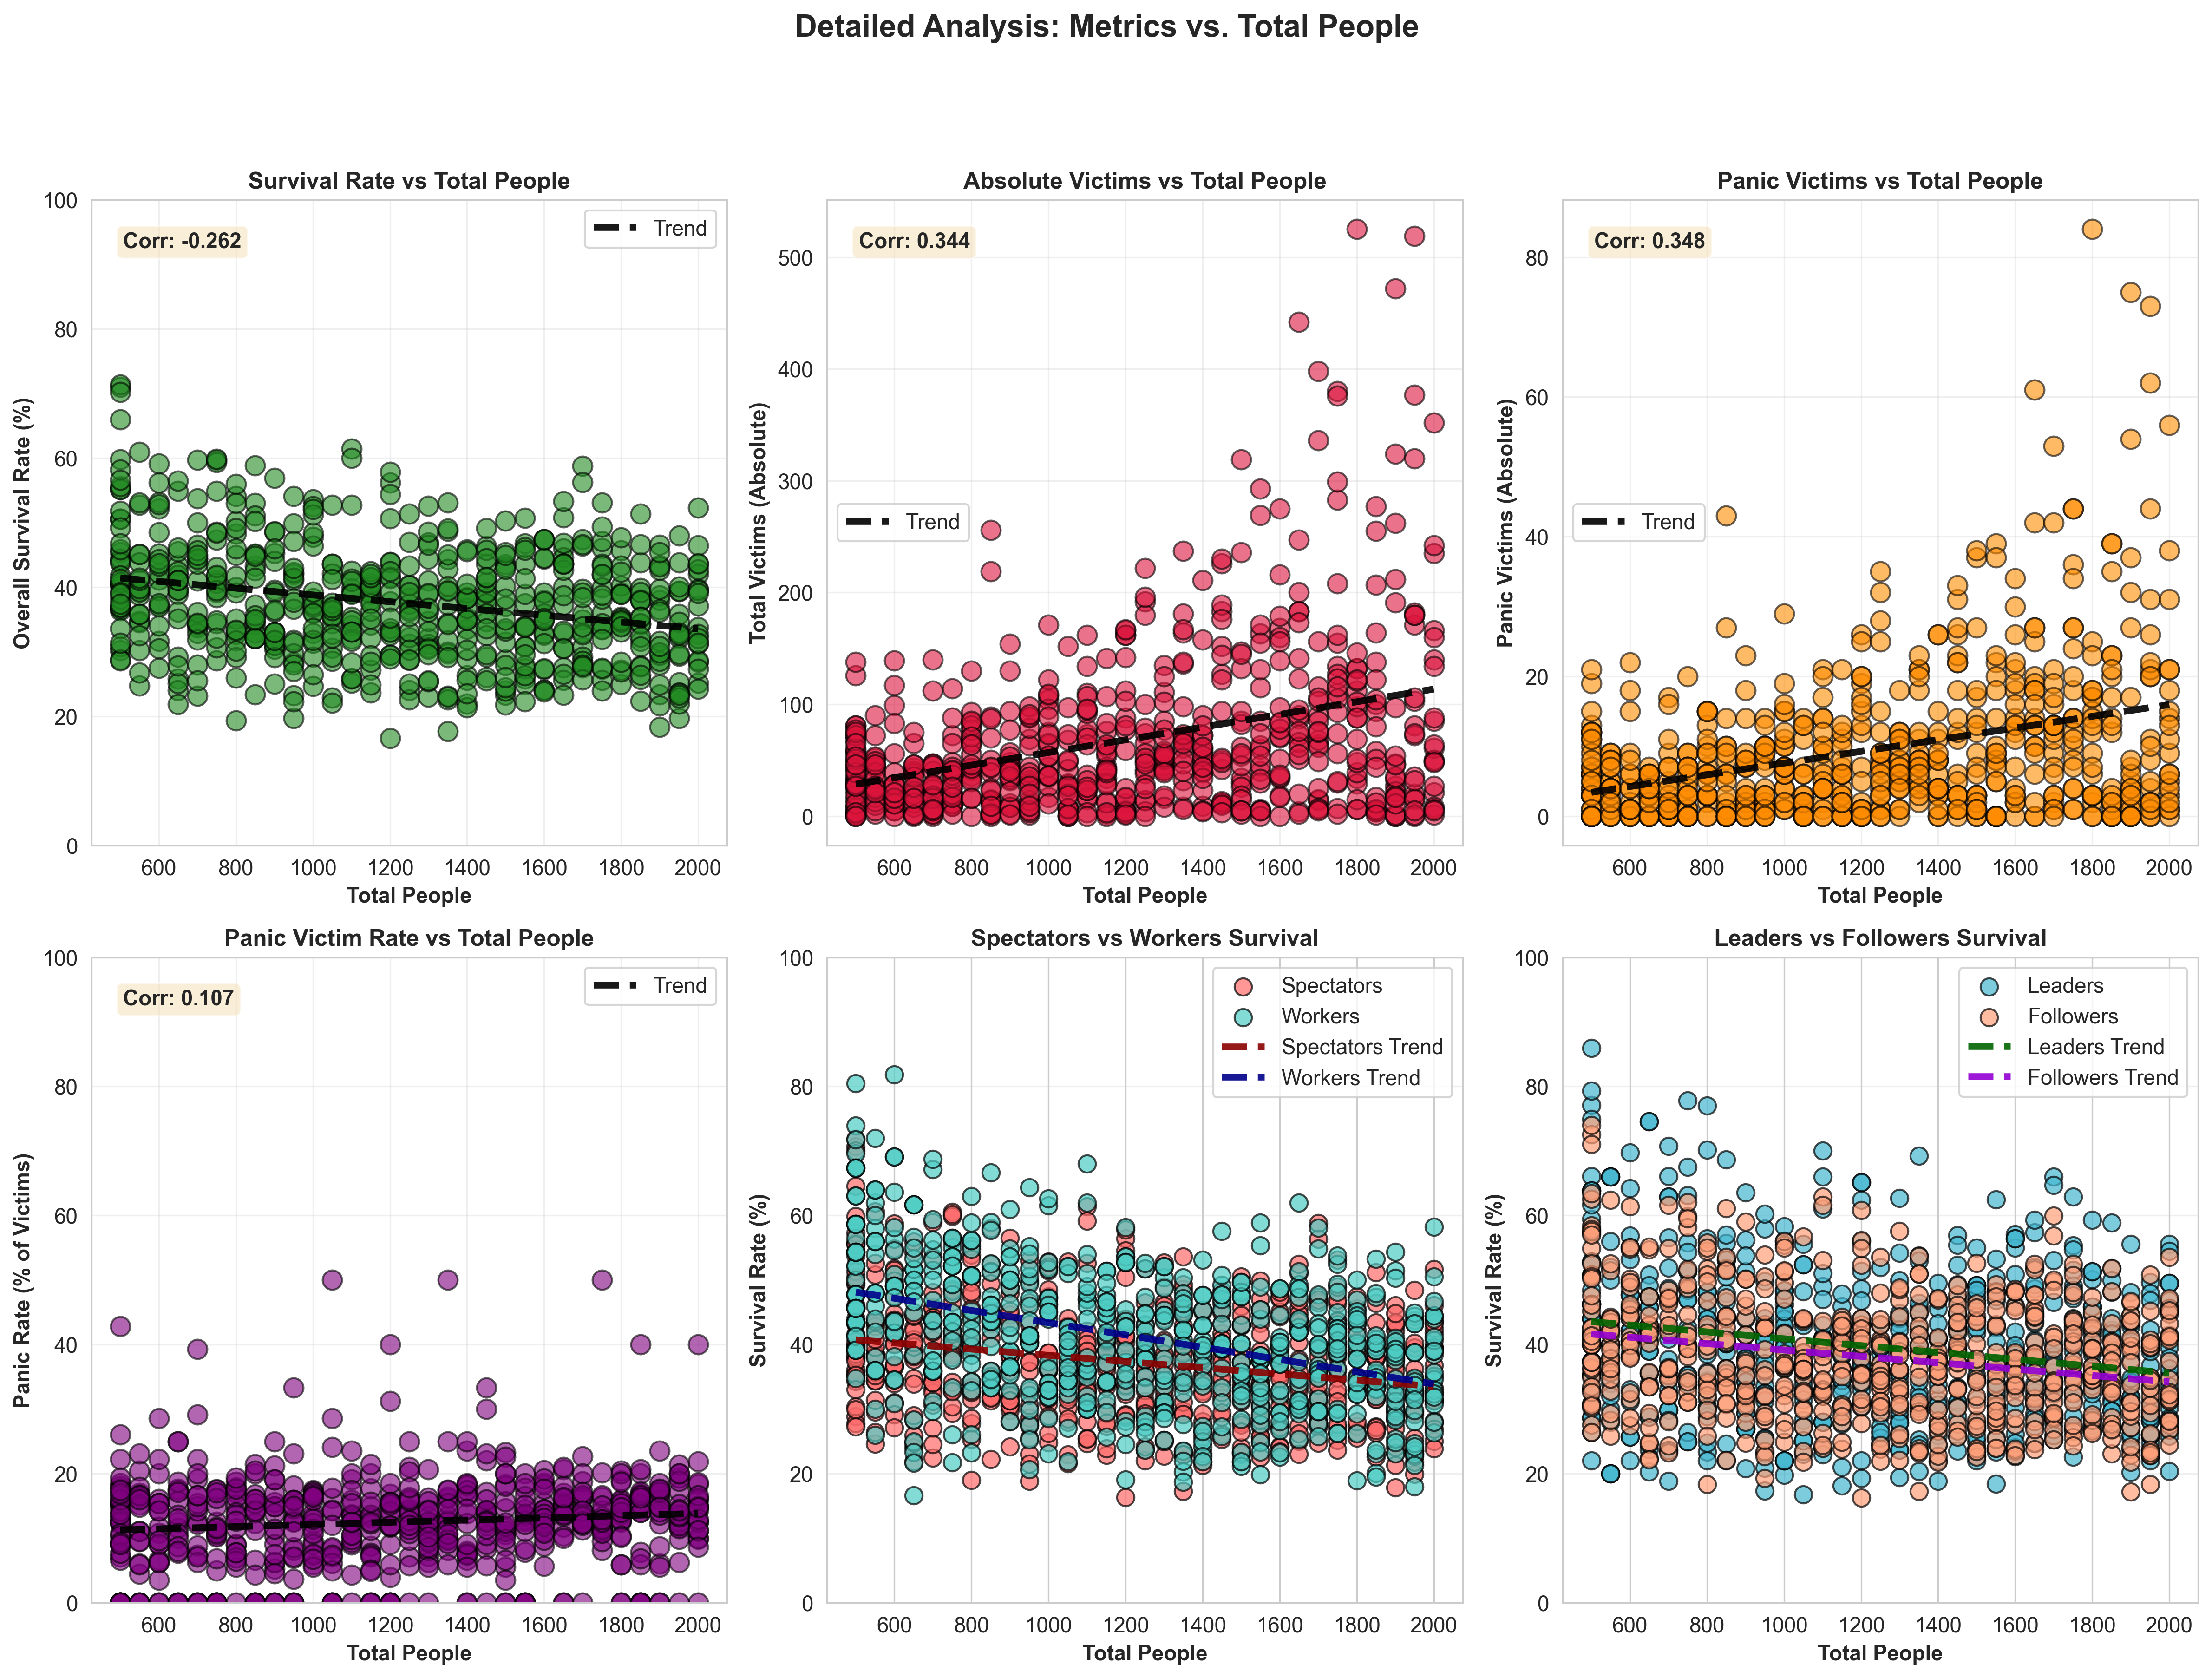
\includegraphics[width=0.9\textwidth]{../analysis/output/5.1.png}
\caption{Impact of crowd density on evacuation outcomes.}
\label{fig:5}
\end{figure}

The results shown in Fig.\ref{fig:5} demonstrate a critical inverse relationship between the total number of people and the efficiency of evacuation, caused by congestion.
\begin{itemize}
    \item Overall Survival Rate:
    \begin{itemize}
        \item The Global Survival rate shows a clear decreasing trend (Correlation: Corr $= -0.262$) ​​as \texttt{tot\_people} increases;
        \item This confirms that increased density reduces the efficiency of evacuation.
    \end{itemize}
    \item Absolute victims:
    \begin{itemize}
        \item The number of Absolute Victims (Total Victims) shows a strong upward trend (Correlation: Corr $= 0.344$), increasing from an average of around $100$ victims with $500$ people to more than $300$ with $2000$ people;
        \item The dispersion of the points is noticeably greater at high densities (close to $2000$), suggesting that under conditions of high congestion, the initial randomness (positions of the agents, location of the fire) has a much more dramatic impact on the final result, leading to collapses in some cases (high points in the graph).
    \end{itemize}
\end{itemize}

The main failure mechanism is increased congestion, influenced by the \texttt{modify\_speed} reflex of the agents, since as the population increases, the number of nearby neighbors increases, which exponentially reduces the speed of the agents, causing greater slowdown and more deaths.

Essentially, the workers are always alert and in a leadership role, giving them a high survival rate even at high density, demonstrating the effectiveness of the staffing policy.
Regarding bystander roles, while the proportion of victims who were panicking shows only a slight upward trend, the crucial absolute number of panicked victims skyrockets with density. This is because panicked agents have a greater perception distance and experience a two-way slowing effect.

\section{Conclusions and Future Work}

This report has presented the \textit{StadiumEvacuation} agent-based model, developed using the GAMA platform, to simulate crowd evacuation dynamics in a stadium environment under the threat of a spreading hazard. The model incorporates heterogeneous agent behaviors, realistic spatial representation from GIS data, and key parameters influencing evacuation outcomes. Through a series of experiments, we have demonstrated how factors such as worker-to-spectator ratio, perception distance, agent speed, hazard spread rate, role composition, and crowd density significantly impact evacuation efficiency and safety. The results highlight the importance of social organization, effective communication, and environmental design in managing crowd evacuations. 

Different enhancements could be made to this model in the future: for example, incorporating more complex agent behaviors (e.g., group dynamics, emotional states), simulating different types of hazards with varying spread patterns, or integrating real-time data inputs to adapt evacuation strategies dynamically. Additionally, further validation against empirical data from real-world evacuations could enhance the model's credibility and applicability for practical safety planning.

\bibliographystyle{splncs04}
\bibliography{references}

\end{document}